\documentclass[UTF8,a4paper]{article}
\usepackage{fancyhdr}
\usepackage{ctex}
\usepackage{CJK}
\usepackage{amsmath}
\usepackage{listings}
\usepackage{graphics}
\usepackage{graphicx}
\usepackage{color}
\usepackage{xcolor}
\usepackage{geometry}
\usepackage{indentfirst}
\setlength{\parindent}{2em}
\geometry{left=1.5cm,right=1.5cm,top=2cm,bottom=1.5cm}
\lstset{breaklines}%这条命令可以让LaTeX自动将长的代码行换行排版
\lstset{extendedchars=false}%这一条命令可以解决代码跨页时,章节标题,页眉等汉字不显示的问题
\lstset{ 
	language=C++,                % choose the language of the code
	basicstyle=\small\sf,    % the size of the fonts that are used for the code
	tabsize=3,                            % sets default tabsize to 3 spaces
	numbers=left,                   % where to put the line-numbers
	numberstyle=\tiny,              % the size of the fonts that are used for the line-numbers
	stepnumber=1,                   % the step between two line-numbers. If it's 1 each line
	% will be numbered
	numbersep=5pt,                  % how far the line-numbers are from the code   %
	keywordstyle=\color[RGB]{33,33,234},               % keywords
	commentstyle=\color[RGB]{0,0,0},    % comments
	stringstyle=\color[rgb]{0.170,0.187,0.102},      % strings
    backgroundcolor=\color{white},
    rulesepcolor=\color[RGB]{20,20,20},  % choose the background color. You must add \usepackage{color}
	showspaces=false,               % show spaces adding particular underscores
	showstringspaces=false,         % underline spaces within strings
	showtabs=false,                 % show tabs within strings adding particular underscores                frame = single,         % adds a frame around the code
	captionpos=b,                   % sets the caption-position to bottom
	breaklines=true,                % sets automatic line breaking
	breakatwhitespace=false,        % sets if automatic breaks should only happen at whitespace
	title=\lstname,                 % show the filename of files included with \lstinputlisting;
	% also try caption instead of title
	mathescape=true,escapechar=?    % escape to latex with ?..?
	escapeinside={\%*}{*)},         % if you want to add a comment within your code
	%columns=fixed,                  % nice spacing
	%morestring=[m]',                % strings
	%morekeywords={%,...},%          % if you want to add more keywords to the set
	%    break,case,catch,continue,elseif,else,end,for,function,global,%
	%    if,otherwise,persistent,return,switch,try,while,...},%
}
\pagestyle{fancy}
\lhead{数据结构作业}
\chead{}
\rhead{\bfseries 22920182204393庄震丰}
\lfoot{}
\cfoot{\thepage}
\rfoot{}
\renewcommand{\headrulewidth}{0.4pt}
\begin{document}
\begin{center}
    \textbf{\LARGE{数据结构作业 第七章——图}}\\[0.5cm]
    \normalsize{庄震丰 22920182204393}\\[0.3cm]
    \large{Nov. $17^{th}$, 2019}
\end{center}
\textbf{7-15}\\
题目要求:试在邻接矩阵存储结构上实现图的基本操作:InsertVex(G,v),InsertArc(G,v,w),DeleteVex(G,v)和DeleteArc(G,v,w)\\
算法分析:插入节点直接在原矩阵的基础上记录出入度信息可以,并且在对角线上标记该点是否存在。插入边v,w,则直接令a(i,j)为边权value即可。删除时相反操作就可以。\\[0.2cm]
空间复杂度$O(n^2)$,时间复杂度$O(m\Delta)$,m是操作数,$\Delta$为最大度。\\
7-15.cpp
\begin{lstlisting}
    #include<bits/stdc++.h>
    using namespace std;
    #define maxn 1000
    #define inf 0x3f3f3f3f
    struct Graph
    {
        int MAP[maxn][maxn];
        int num;
    }G;
    void InsertVex(Graph &G,int v)
    {
        int n;
        G.num++;
        int x,value;
        cout<<"input the indegree number:"<<endl;
        cin>>n;
        cout<<"input the point and value"<<endl;
        for (int i=1;i<=n;i++)
            {
                cin>>x>>value;
                G.MAP[v][x]=value;
            }
        cout<<"output the indegree number:"<<endl;
        cin>>n;
        cout<<"input the point and value"<<endl;
        for (int i=1;i<=n;i++)
            {
                cin>>x>>value;
                G.MAP[x][v]=value;
            }
    }
    void InsertArc(Graph &G,int v,int w)
    {
        cout<<"please input the value"<<endl;
        int value;
        cin>>value;
        G.MAP[v][w]=value;
    }
    void DeleteVex(Graph &G,int v)
    {
        G.num--;
        for (int i=0;i<maxn;i++)
        {
            G.MAP[i][v]=inf;
            G.MAP[v][i]=inf;
        }
    }
    void DeleteArc(Graph &G,int v,int w)
    {
        G.MAP[v][w]=inf;
    }
    void init()
    {
        for (int i=0;i<maxn;i++)
            for (int j=0;j<maxn;j++)
                G.MAP[i][j]=inf;
    }
    void print()
    {
        for (int i=1;i<=G.num;i++)
            {
            for (int j=1;j<=G.num;j++)
                cout<<G.MAP[i][j]<<" ";
                cout<<endl;
            }
    }
    void operat()
    {
        int type,p,q;
        cin>>type;
        while(type!=-1)
        {
            if(type==1)
            {
                cout<<"Insert point:"<<endl;
                cin>>p;
                InsertVex(G,p);
            }
            if(type==2)
            {
                cout<<"Insert Arc:"<<endl;
                cin>>p>>q;
                InsertArc(G,p,q);
            }
            if(type==3)
            {
                cout<<"Delete point:"<<endl;
                cin>>p;
                DeleteVex(G,p);
            }
            if(type==4)
            {
                cout<<"Delete Arc:"<<endl;
                cin>>p>>q;
                DeleteArc(G,p,q);
            }
            if (type==5)
            {
                cout<<"Matrix is:"<<endl;
                print();
            }
            cin>>type;
        }
    }
    int main()
    {
        init();
        operat();
        print();
        return 0;    
    }
\end{lstlisting}
\textbf{7-16}\\
题目要求:利用邻接表实现7-15题的操作。\\
算法分析:邻接表重新构造图的结构体,每个点建立vector储存每个点的出度点。\\
插入操作时,每得到一个后继点就插入当前点的vector,每得到一个入度点,就将当前点插入到每个前驱点的vector。插入边的操作就是直接将w插入到vector[v]中。\\
值得注意的是,当进行删除操作点操作时,除了删除当前点出度点之外,也要删除所有其他点出度为当前点的边。
空间复杂度$O(E)$,插入边为O(1),插入点最多为O(N),设操作数为M,则时间复杂度O(MN).\\
7-16.cpp\\
\begin{lstlisting}
    #include<bits/stdc++.h>
    using namespace std;
    #define maxn 1000
    #define inf 0x3f3f3f3f
    struct Graph
    {
        vector<int> Link[maxn];
        int num;
    }G;
    void InsertVex(Graph &G,int v)
    {
        int n;
        G.num++;
        int x;
        cout<<"input the indegree number:"<<endl;
        cin>>n;
        for (int i=1;i<=n;i++)
            {
                cin>>x;
                G.Link[x].push_back(v);
            }
        cout<<"output the indegree number:"<<endl;
        cin>>n;
        for (int i=1;i<=n;i++)
            {
                cin>>x;
                G.Link[v].push_back(x);
            }
    }
    void InsertArc(Graph &G,int v,int w)
    {
        G.Link[v].push_back(w);
    }
    void DeleteVex(Graph &G,int v)
    {
        
        while(!G.Link[v].empty())
        {
            G.Link[v].pop_back();
        }
        for (int i=1;i<=G.num;i++)
        {
            vector<int>::iterator it;
            it=find(G.Link[i].begin(),G.Link[i].end(),v);
            G.Link[i].erase(it);
        }
    G.num--;
    }
    void DeleteArc(Graph &G,int v,int w)
    {
        vector<int>::iterator it;
      v  it=find(G.Link[v].begin(),G.Link[v].end(),w);
        G.Link[v].erase(it);
    }
    void operat()
    {
        int type,p,q;
        cin>>type;
        while(type!=-1)
        {
            if(type==1)
            {
                cout<<"Insert point:"<<endl;
                cin>>p;
                InsertVex(G,p);
            }
            if(type==2)
            {
                cout<<"Insert Arc:"<<endl;
                cin>>p>>q;
                InsertArc(G,p,q);
            }
            if(type==3)
            {
                cout<<"Delete point:"<<endl;
                cin>>p;
                DeleteVex(G,p);
            }
            if(type==4)
            {
                cout<<"Delete Arc:"<<endl;
                cin>>p>>q;
                DeleteArc(G,p,q);
            }
            cin>>type;
        }
    }
    int main()
    {
        operat();
        return 0;
    }    
\end{lstlisting}
\textbf{7-25}\\
题目要求:假设对有向图中n个顶点进行自然编号,并以三个数组$s[1\cdots max],fst[1\cdots n],lst[1\cdots n]$表示之。其中数组s存放每个顶点后继顶点的信息,第i个顶点后继存放在s中下标从fst[i],lst[i]的分量中(i=1,2,...,n)。若fst[i]>lst[i],则第i个顶点无后继顶点。试编写判别该有向图中是否存在回路的算法。\\
算法分析:首先进行预处理,得到所有节点的入度:对s进行扫描。将fst[i]...lst[i]中点入度+1。\\
得到所有点的入度后,进行以下操作:
\begin{itemize}
    \item 找到没有入度为零的节点,删除之,将其后继节点的入读全部减去1,同时将图中的点计数器-1。
    \item 当找不到入度为0的点的时候,退出,否则重复以上操作。
    \item 退出后如果还有一个点,判断它有没有自环,如果没有自环就删除该点,计数器-1。
    \item 当点计数器大于零,则存在回路,若为0则不存在回路。
\end{itemize}
以上为拓扑思路。\\
空间复杂度:$O(n)$,时间复杂度$O(E)$\\
7-25.cpp\\
\begin{lstlisting}
    #include<bits/stdc++.h>
    using namespace std;
    #define maxn 1000
    #define inf 0x3f3f3f3f
    int s[maxn];
    int pre[maxn]={0};
    int fst[maxn],lst[maxn];
    int n;
    void init()
    {
        for (int i=0;i<maxn;i++)
        {
            fst[i]=-1;lst[i]=-1;
        }
    }
    bool fin()
    {
        for (int i=1;i<=n;i++)
        {
            if (pre[i]==0) return i;
        }
        return -1;
    }
    int main()
    {
        cin>>n;
        for (int i=1;i<=n;i++)
            cin>>s[i];
        for (int i=1;i<=n;i++)
            cin>>fst[i];
        for (int i=1;i<=n;i++)
            cin>>lst[i];
        for (int i=1;i<=n;i++)
            for (int j=fst[i];j<=lst[i];j++)
                pre[j]++;
        int N=n;
        int k=fin();
        while(k)
        {
            N--;
            for (int j=fst[k];j<=lst[k];j++)
                pre[j]--;//拓扑删点
            k=fin();
        }
        if (N>0) cout<<"YES"; else cout<<"NO";
        return 0;
    }      
\end{lstlisting}
\newpage
\textbf{Sample}\\[1cm]
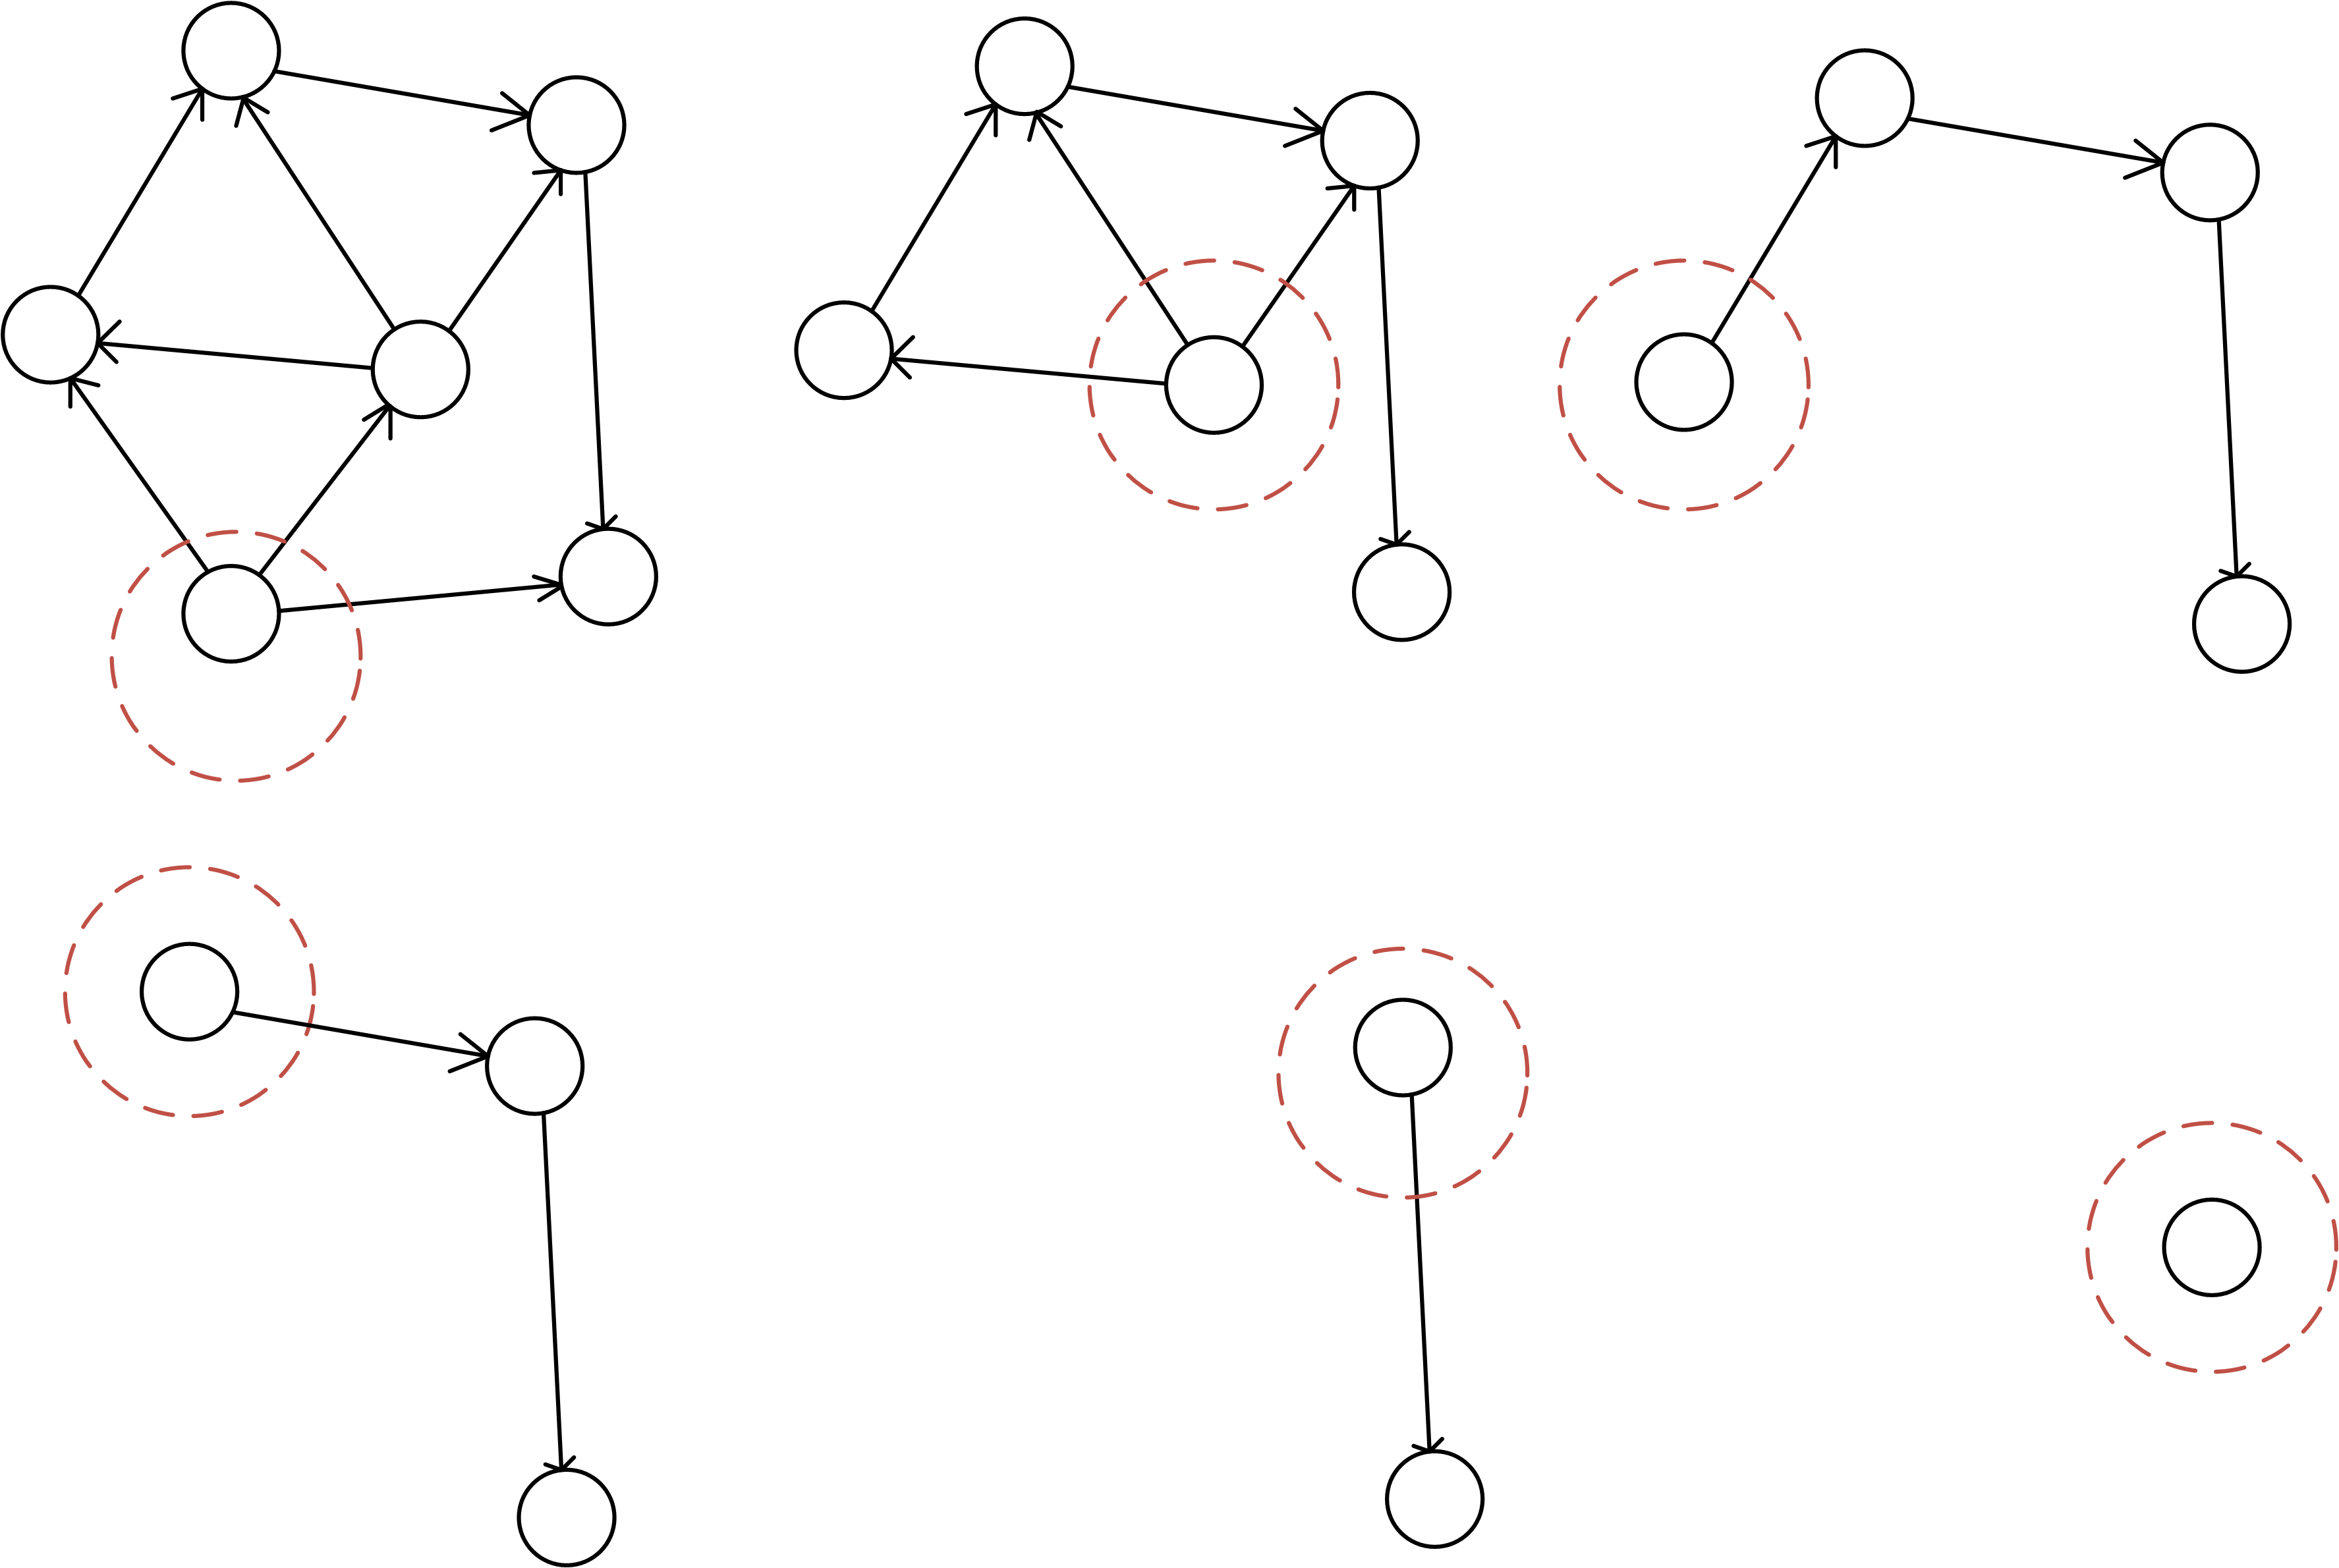
\includegraphics[scale=1]{7-25.png}\\
\textbf{7-27}\\
题目要求:采用邻接表结构,编写一个判别无向图中任意两点是否一条长为k的简单路径的算法。\\
算法分析:DFS。从起点开始深搜,每当搜到无出度的点或者长度(搜索深度)大于K,则return,否则沿着后继点一直进行,找到在全局变量标记。\\
算法复杂:空间复杂度$O(E)$,时间复杂度$O(E)$\\
7-27.cpp
\begin{lstlisting}
    #include<bits/stdc++.h>
    using namespace std;
    #define maxn 1000
    #define inf 0x3f3f3f3f
    int n,k,v,w;
    int flag=false;
    struct Graph
    {
        vector<int> Link[maxn];
        int num;
    }G;
    bool vis[maxn];
    void dfs(int x,int deep)
    {
        if(x==w&&deep==k) 
         {
            flag=true;
            return;
         }
         for (vector<int>::iterator it=G.Link[x].begin();it!=G.Link[x].end();it++)
            {
                vis[*it]=true;
                dfs(*it,deep+1);
                vis[*it]=false;
            }
        return;
    }
    void init()
    {
        int m,p;
        cin>>n;
        for (int i=1;i<n;i++)
        {
            cin>>m;
            for (int j=1;j<=m;j++)
            {
                cin>>p;
                G.Link[i].push_back(j);
            }
        }
        memset(vis,sizeof(vis),false);
    }
    int main()
    {
        cin>>v,w,k;
        init();
        dfs(v,1);
        if (flag) cout<<"Exist";else cout<<"Not Exist";
    }    
\end{lstlisting}
\textbf{7-33}
题目要求:已知一无向图边集保存在某个类型EdgeSetType的数据结构EdgeSet中,并在此结构上已定义两种基本运算:
\begin{itemize}
    \item 函数GetMinEdge(EdgeSet,u,v):若EdgeSet非空,则必存在最小边,变参u和v的最小边上两个顶点,并返回true,否则返回false
    \item 过程DelMinEdge(EdgeSet,u,v):从EdgeSet中删除依附于顶点u和v的最小边。 
\end{itemize}
算法分析:先建立EdgeSet结构体,读入初始信息,用数组建立边,GetMinEdge函数就利用其进行遍历,记录下最小边的序号,并判断两点是否为u和v。\\
Del函数也是进行遍历,若E<u,v>存在,则删除,可以直接用结构体中的bool变量进行标记。\\
空间复杂度O(E),两个函数的时间复杂度O(E)\\
7-36.c
\begin{lstlisting}

    #include <stdio.h>

    /* 类型定义 */
    typedef int MFSet; 						//并查集 
    typedef	struct							//边的集合 
    {
        int u, v;							//端点 
        int Weight;							//权值 
    }EdgeSetType;
    typedef	struct							//不带权值的边的集合 
    {
        char u;
        char v;								//端点 
    }Edge;
    
    /* 函数原型 */
    CSTree MinSpanTree_KRUSKAL_7_33(ALGraph G);
    void InitEdgeSet_7_33(EdgeSetType EdgeSet[], ALGraph G);		//初始化边集 
    Status GetMinEdge_7_33(EdgeSetType EdgeSet[], int *u, int *v);	//获取最小边<u, v>
    void DelMinEdge_7_33(EdgeSetType EdgeSet[], int u, int v);		//删除边<u, v> 
    void InitMFSet_7_33(MFSet S[], ALGraph G);						//初始化并查集 
    int FindSeat_7_33(MFSet S[], int u);							//返回顶点u所在集合 
    void Merge_7_33(MFSet S[], int u, int v);						//将集合u并入集合v 
    CSTree CreateCSTree_7_33(Edge E[]);								//根据边集创建树 
    void AddEdgeToTree_7_33(CSTree *T, char v, char w);				//添加边<v,w>到树中,v为连接点
    
    int main(int argc, char *argv[])
    {
        ALGraph G;
        FILE *fp;										//作为输入源
        CSTree T;
    
        printf("创建并输出无向图(带权)...\n");	
        fp = fopen("Data/Algo_7_33.txt", "r");
        CreateGraph_AL(fp, &G); 
        fclose(fp);
        OutputALGraph(G);
        printf("\n");	
        
        T= MinSpanTree_KRUSKAL_7_33(G);
        printf("此无向连通网的最小生成树为:\n");
        Print_CS(T);
        printf("\n");
    }
    
    CSTree MinSpanTree_KRUSKAL_7_33(ALGraph G)			//假设图的权值均大于0 
    {
        MFSet S[G.vexnum+1];							//并查集 
        EdgeSetType EdgeSet[G.arcnum+1];				//原始边集 
        Edge E[G.vexnum];								//筛选后的最小边集								
        int u, v;
        int k;
        
        InitEdgeSet_7_33(EdgeSet, G);
        InitMFSet_7_33(S, G);
        
        k = 1;
        E[0].u = E[0].v = G.vexnum-1;
        
        while(k<=G.vexnum-1)
        {
            if(GetMinEdge_7_33(EdgeSet, &u, &v))				//找到最小边 
            {
                if(FindSeat_7_33(S, u)!=FindSeat_7_33(S, v))	//判断是否构成回路 
                {
                    E[k].u = G.vertices[u].data;
                    E[k].v = G.vertices[v].data;
                    Merge_7_33(S, u, v);						
                    k++;
                }
            
                DelMinEdge_7_33(EdgeSet, u, v); 
            }
        }
        
        return CreateCSTree_7_33(E);
    }
    
    void InitEdgeSet_7_33(EdgeSetType EdgeSet[], ALGraph G)
    {
        int k, count;
        ArcNode *r;
        
        EdgeSet[0].Weight = G.arcnum;
        
        for(k=1,count=0; k<=G.vexnum; k++)
        {
            r = G.vertices[k].firstarc;
            while(r && r->adjvex<k)
                r = r->nextarc;
            while(r)
            {
                count++;
                EdgeSet[count].u = k;
                EdgeSet[count].v = r->adjvex;
                EdgeSet[count].Weight = r->info.in;
                r = r->nextarc;
            }
        }
    }
    
    Status GetMinEdge_7_33(EdgeSetType EdgeSet[], int *u, int *v)
    {
        int k;
        int min = INT_MAX;
        
        for(k=1; k<=EdgeSet[0].Weight; k++)
        {
            if(EdgeSet[k].Weight<min)
            {
                min = EdgeSet[k].Weight;
                *u = EdgeSet[k].u;
                *v = EdgeSet[k].v;
            }
        }
        
        if(min==INT_MAX)
            return ERROR;
        else
            return OK;
    }
    
    void DelMinEdge_7_33(EdgeSetType EdgeSet[], int u, int v)
    {
        int k;
        
        for(k=1; k<=EdgeSet[0].Weight; k++)
        {
            if((EdgeSet[k].u==u&&EdgeSet[k].v==v) || (EdgeSet[k].u==v&&EdgeSet[k].v==u))
            {
                while(k+1<=EdgeSet[0].Weight)
                {
                    EdgeSet[k] = EdgeSet[k+1];
                    k++;
                }
                
                break;
            }	
        }
        
        EdgeSet[0].Weight--;
    }
    
    void InitMFSet_7_33(MFSet S[], ALGraph G)
    {
        int k;
        
        S[0] = G.vexnum;
        
        for(k=1; k<=G.vexnum; k++)
            S[k] = -1;
    }
    
    int FindSeat_7_33(MFSet S[], int u)
    {
        int k;
        
        for(k=u; S[k]>0; k=S[k])
            ;
        
        return k;
    }
    
    void Merge_7_33(MFSet S[], int u, int v) //集合u合并到集合v 
    {
        int k;
        
        S[u] = v;
        
        for(k=v; S[k]>0; k=S[k])
            ;
                
        S[k]--;
    }
    
    CSTree CreateCSTree_7_33(Edge E[])
    {
        CSTree T;
        char Stack[E[0].u+1];					//模拟栈 
        int i, j, k;
        char tmp;
        
        InitTree_CS(&T);						//初始化孩子-兄弟树 
        k = -1;
        
        if(E[0].u)								//边集不为空
        {
            Stack[++k] = E[1].v;
            Stack[++k] = E[1].u;
            AddEdgeToTree_7_33(&T, E[1].u, E[1].v);
            
            while(k>=0)
            {
                tmp = Stack[k--];
                for(i=2; i<=E[0].u; i++)
                {
                    if(E[i].u==tmp || E[i].v==tmp)
                    {
                        if(E[i].u==tmp)
                        {
                            AddEdgeToTree_7_33(&T, E[i].u, E[i].v);
                            Stack[++k] = E[i].v;		
                        }
                        else
                        {
                            Stack[++k] = E[i].u;
                            AddEdgeToTree_7_33(&T, E[i].v, E[i].u);				
                        }
                            
                        E[i].u = E[i].v = '\0';		//相当于删掉此条已访问过的边 
                    }
                }
            }		
        } 
        
        return T;	
    }
    
    void AddEdgeToTree_7_33(CSTree *T, char v, char w)
    {
        CSTree p, q, r;
        
        r = (CSTree)malloc(sizeof(CSNode));
        r->data = w;
        r->firstchild = r->nextsibling = NULL;
        
        if(!(*T))
        {
            *T = (CSTree)malloc(sizeof(CSNode));
            (*T)->data = v;
            (*T)->firstchild = r;
            (*T)->nextsibling = NULL;		
        }
        else
        {
            p = Order_CS(*T, v);
            q = p->firstchild;
            
            if(!q)
                p->firstchild = r;
            else
            {
                while(q && q->nextsibling)
                    q = q->nextsibling;
                q->nextsibling = r;	
            }
        }
    }    
\end{lstlisting}
\textbf{7-36}\\
题目要求:在图的邻接表存储结构中,为每个定点增加一个MPL域,试写一算法,求有向无环图G的每个顶点出发的最长路径的长度,并把它存进MPL域,给出算法复杂度。\\
算法分析:FLOYD.首先将邻接存储结构化为邻接矩阵,减少访问边权时间。利用FLOYD求出所有点的最长路。\\
再对每个点进行遍历,得到最长distance,将其push进MPL域。\\
空间复杂度$O(E+N^2)$,时间复杂度$O(N^3)$\\
7-36.cpp\\
\begin{lstlisting}
    #include<bits/stdc++.h>
    #define MAX 1000000000
    using namespace std;
    int d[1000][1000],path[1000][1000];//FLOYD
    vector<int> MPL;
    int main()
    {
        int i,j,k,m,n;
        int x,y,z;
        scanf("%d%d",&n,&m);
        for(i=1;i<=n;i++)
            for(j=1;j<=n;j++)
            {
                d[i][j]=MAX;
                path[i][j]=j;
            }
        for(i=1;i<=m;i++)
        {
                scanf("%d%d%d",&x,&y,&z);
                d[x][y]=z;
                d[y][x]=z;
        }
        for(k=1;k<=n;k++)
            for(i=1;i<=n;i++)
                for(j=1;j<=n;j++) {
                    if(d[i][k]+d[k][j]<d[i][j]) {
                        d[i][j]=d[i][k]+d[k][j];
                        path[i][j]=path[i][k];
                    }
                }
        for(i=1;i<=n;i++)
            for(j=i+1;j<=n;j++)
              if (i!=j) printf("%d->%d:%d\n",i,j,d[i][j]);
        int f, en;
        scanf("%d%d",&f,&en);
        while (f!=en)
        {
            printf("%d->",f);
            f=path[f][en];
        }
        printf("%d\n",en);
        for (int i=1;i<=n;i++)
        {
            int t=-MAX,fl=1;
            for (int j=1;j<=n;j++)
            {
                if (d[i][j]!=MAX)
                {
                    if (d[i][j]>t) 
                    {
                        t=d[i][j];
                        fl=j;
                    }
                }
            }
            MPL.push_back(fl);
        }
        return 0;
    }     
\end{lstlisting}
\end{document}